\chapter{Bibliotecas de programación orientadas al web scraping}
\label{cha:bibliotecas de programacion orientadas al web scraping}

\section{Búsqueda de bibliotecas destinadas al web scraping}
\label{sec:busqueda de bibliotecas destinadas al web scraping}

Como se especificó en la sección \ref{sec:objetivo y limitaciones} este trabajo se limitará a realizar
una comparativa de los programas software de minado web más frecuentes. Esta comparativa se efectúa con el
fin de conocer cuál o cuáles de estos programas o paquetes software son los más rentables para este propósito.

¿Como saber que paquetes software destinados al minado web son los más comunes? Durante todo este capítulo
se procederá a la búsqueda, selección e introducción de programas software empleados para el \emph{web 
scraping}. Cabe destacar que Python y R serán los lenguajes de programación con los que se trabajará tanto 
para el desarrollo de la herramienta de comparación, como para el proceso de extracción de datos.

El primer paso consiste en buscar todos los elementos posibles que conforman la población de paquetes
software del mercado, ya sean de Python o R. La búsqueda de estos paquetes se ha realizado a través de las 
distintas fuentes de información mostradas a continuación:

\begin{enumerate}
  \item GitHub \cite{github}. Gran parte de los desarrolladores de estos programas, publican su trabajo en
  estos repositorios de código abierto.
  \item CRAN \cite{cran}. The Comprehensive R Archive Network es una red de servidores ftp y web que
  almacena versiones idénticas de código y documentación para R.
  \item PyPi \cite{pypi}. Python Package Index es un repositorio de software para Python, útil para la
  búsqueda de paquetes de un determinado propósito.
\end{enumerate}

\section{Bibliotecas de Python encontradas durante el proceso de búsqueda}
\label{sec:bibliotecas de python encontradas durante el proceso de busqueda}

A continuación, se hará una breve sinopsis de las bibliotecas de Python encontradas. Esta sinopsis tiene 
como objetivo conocer el funcionamiento, funciones principales y proceso de extracción de las mismas.

Es posible que algunos de los paquetes hayan sido desarrollados tanto en R como en Python. En ese caso, por 
un lado, la introducción se realzará de forma conjunta, sin embargo, será interesante ver el código del 
mismo en ambos casos y como se comportan estos ante los distintos test de evaluación.

Antes de comenzar con la sinopsis de bibliotecas, es conveniente revisar el apéndice \ref{cha:analizadores 
empleados en los paquetes de web scraping}, donde se realiza una breve introducción de aquellos analizadores 
empleados en las mismas. Los 'emparejamientos' entre biblioteca-analizador se recogen en la tabla 
\ref{tab:emparejamientos biblioteca-analizador} a modo de resumen.

\begin{table}[h]
  \begin{center}
  \begin{tabular}{| c | c | c | c | c | c | c |} \hline 
    \textbf{inscriptis} & \textbf{dragnet} & \textbf{boilerpy} & \textbf{libextract} & \textbf{news-please} & \textbf{justext} & \textbf{goose3} \\ \hline
    lxml & lxml & html parser & lxml & lxml & lxml & lxml \& html parser \\ \hline
  \end{tabular}

  \hfill \break

  \begin{tabular}{| c | c | c | c | c | c |} \hline 
    \textbf{html2text} & \textbf{readability} & \textbf{trafilatura} & \textbf{beautiful soup} & \textbf{newspaper3k} & \textbf{html\_text}  \\ \hline
    html parser & lxml & lxml & lxml \& html5lib \& html & lxml & lxml \\ \hline
  \end{tabular}

  \caption{Emparejamientos biblioteca-analizador}
  \label{tab:emparejamientos biblioteca-analizador}
  \end{center}
\end{table}

Ya sea porque determinadas bibliotecas permiten al desarrollador seleccionar entre varios tipos de 
analizadores, o bien porque múltiples de ellos son necesarios para el correcto funcionamiento de la 
extracción, muchas de estas bibliotecas hacen uso de más de un analizador en su código.

\subsection{inscriptis}
\label{subsec:inscriptis}

Además de ser una biblioteca de conversión de HTML a texto basada en Python, \textbf{inscriptis} 
\cite{inscriptis} también tiene soporte como línea de comandos o como servicio web para tablas anidadas. 
A pesar de sus múltiples funcionalidades esta sección se centra en \textbf{inscriptis} como biblioteca de 
programación.

\subsubsection{Estructura de la solución}
\label{subsubsec:estructura de la solucion}

A diferencia de otros algoritmos de extracción, \textbf{inscriptis} no solo tiene en cuenta la calidad del 
texto extraído, la estructura del mismo también es muy importante. Esto provoca que el resultado obtenido 
se acerque más a un posible resultado aplicando el método tradicional a través de cualquier navegador web.

Se muestra a continuación una pequeña comparación entre la extracción de texto de \textbf{Beautiful Soup}
\ref{subsec:beautiful soup}, con la extracción de texto de \textbf{inscriptis}, donde se tiene un fragmento 
HTML como el siguiente como objeto de prueba.

\begin{Schunk}
  \begin{Soutput}
      <li>first</li>
      <li>second</li>
  \end{Soutput}
\end{Schunk}

Se emplea en primer lugar el método \emph{get\_text()} propio de \textbf{Beautiful Soup} sobre el fragmento 
HTML anterior.

\begin{Schunk}
  \begin{Soutput}
    # firstsecond
  \end{Soutput}
\end{Schunk}

Se puede observar que el formato obtenido no es el adecuado, puesto que no se ha respetado la estructura
del documento base. Sin embargo, si se aplica \textbf{inscriptis} sobre el mismo fragmento HTML, la salida 
obtenida sería la siguiente:

\begin{Schunk}
  \begin{Soutput}
    # first
    # second
  \end{Soutput}
\end{Schunk}

El algoritmo no solo admite construcciones tan simples como la anterior, también es posible analizar 
construcciones mucho más complejas, como las tablas anidadas, y subconjuntos de atributos HTML o CSS donde 
es esencial una conversión precisa de HTML a texto.

\subsubsection{Reglas de anotación}
\label{subsubsec:reglas de anotacion}

La técnica que se emplea en este caso se conoce como reglas de anotación, es decir, mapeos que permiten 
realizar anotaciones sobre el texto extraído. Estas anotaciones se basan en la información estructural y 
semántica codificada en las etiquetas y atributos HTML utilizados para controlar la estructura y diseño 
del documento original. Con el fin de asignar etiquetas y/o atributos HTML a las anotaciones, se utiliza 
lo que se conoce como perfil de anotaciones, algo parecido a un diccionario. 


\begin{table}[h]
  \begin{center}
  \begin{tabular}{| c | c |} \hline 
    h1 & ['heading', 'h1'] \\ \hline
    h2 & ['heading', 'h2'] \\ \hline
    b & ['emphasis'] \\ \hline
    div\#class=toc & ['table-of-contents'] \\ \hline
    \#class=FactBox & ['fact-box'] \\ \hline
    \#cite & ['citation'] \\ \hline
  \end{tabular}
  \caption{inscriptis - Perfil de anotaciones}
  \label{tab:inscriptis - perfil de anotaciones}
  \end{center}
\end{table}

Si observamos el diccionario mostrado en la tabla \ref{tab:inscriptis - perfil de anotaciones}, las 
etiquetas de tipo cabecera producen anotaciones de tipo \emph{hn}, una etiqueta \emph{<div>} con una 
clase que contiene el valor \emph{toc} da como resultado la anotación \emph{table-of-contents}, y todas 
las etiquetas con un atributo \emph{cite} se anotan como \emph{citation}.

A modo de ejemplo, y con el fin de mostrar el correcto etiquetado del algoritmo, imaginemos que se dispone 
el fragmento de un documento HTML como el mostrado a continuación y unas reglas de anotación como las 
mostradas en la tabla \ref{tab:inscriptis - perfil de anotaciones}.

\begin{Schunk}
  \begin{Soutput}
    <h1>Chur</h1>
    <b>Chur</b> is the capital and largest town of the Swiss 
    canton of the Grisons and lies in the Grisonian Rhine Valley.
  \end{Soutput}
\end{Schunk}

A partir de este ejemplo, y basándonos en el diccionario anterior, la salida esperada debería ser una 
etiqueta de cabecera y otra de énfasis, veamos el resultado que proporciona el proceso de asignación.

\begin{Schunk}
  \begin{Soutput}
    {
      "text": "Chur\n\nChur is the capital and largest town of the Swiss 
              canton of the Grisons and lies in the Grisonian Rhine Valley.",
      "label": [[0, 4, "heading"], [0, 4, "h1"], [6, 10, "emphasis"]]
    }
  \end{Soutput}
\end{Schunk}

Como era de esperar la obtención del texto es precisa, pero no solo del texto sino de su estructura. Además,
la asignación de etiquetas también se ha realizado de forma correcta. Se muestra en el fragmento de código
\ref{cod:inscriptis - uso de reglas de anotacion} como se pueden emplear las reglas de anotación dentro de 
un programa.

\begin{codefloat}
  \inputencoding{latin1}
  \lstinputlisting[style=CppExample]{scripts/inscriptis-reglas-anotacion.py}
  \inputencoding{utf8}
  \caption{inscriptis - Uso de reglas de anotación}
  \label{cod:inscriptis - uso de reglas de anotacion}
\end{codefloat}

\subsubsection{Postprocesamiento}
\label{subsubsec:postprocesamiento}

Además, \textbf{inscriptis} da la posibilidad al usuario de realizar una fase de postprocesamiento donde 
las anotaciones se realizan en un formato determinado. Un primer tipo de postprocesamiento es el que se 
conoce como \emph{surface}, donde se retorna una lista de mapeos entre la superficie de anotación y su 
etiqueta.

\begin{Schunk}
  \begin{Soutput}
    [['heading', 'Chur'],
      ['emphasis': 'Chur']]
  \end{Soutput}
\end{Schunk}

En segundo lugar, el postprocesamiento tipo xml retorna una etiqueta de versión adicional, propia de un
documento XML convencional.

\begin{Schunk}
  \begin{Soutput}
    <?xml version="1.0" encoding="UTF-8" ?>
    <heading>Chur</heading>

    <emphasis>Chur</emphasis> is the capital and largest town of the 
    Swiss canton of the Grisons and lies in the Grisonian Rhine Valley.
  \end{Soutput}
\end{Schunk}

Por último, el postprocesamiento en tipo html crea un documento HTML que contiene el texto convertido y 
resalta todas las anotaciones. Se muestra en la figura \ref{img: inscriptis - postprocesamiento html} un 
ejemplo de la salida obtenida.

\begin{figure}[tphb]
  \centering
  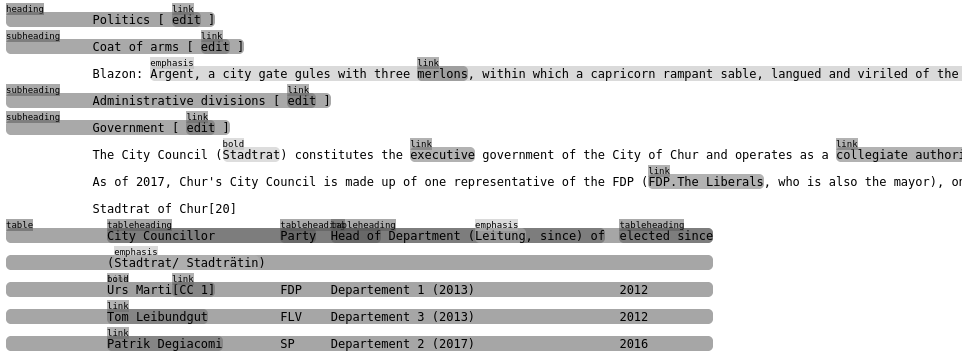
\includegraphics[width=6.3in]{inscriptis-html-postprocessor.png}
  \caption{inscriptis - Postprocesamiento html}
  \label{img: inscriptis - postprocesamiento html}
\end{figure}

\subsection{Beautiful Soup}
\label{subsec:beautiful soup}

Una de las bibliotecas de Python más comunes en el ámbito del \emph{web scraping} es \textbf{Beautiful Soup}
\cite{beautifulsoup}, la cual está diseñada para extraer datos de documentos XML y HTML. Como se muestra
en la tabla \ref{tab:emparejamientos biblioteca-analizador} y a diferencia del resto de bibliotecas,
\textbf{Beautiful Soup} permite determinar el tipo de analizador que se empleará en la extracción, lo que
flexibiliza el proceso de navegación, búsqueda y modificación de documentos.

\subsubsection{Multiplicidad de analizadores}
\label{subsubsec:multiplicidad de analizadores}

\textbf{Beautiful Soup} tiene a \emph{html.parse} como analizador estándar de documentos HTML, pero admite 
varios analizadores de terceros. En la tabla \ref{tab:beautiful soup - analizadores disponibles} se muestran 
los distintos analizadores disponibles, así como un pequeño resumen de las ventajas y desventajas de estos.

\begin{table}[h]
  \begin{center}
  \begin{tabular}{| c | c | c | c |}
  \hline \textbf{Tipo de analizador} & \textbf{Forma de uso} & \textbf{Ventajas} & \textbf{Desventajas} \\ \hline
  html & bs(markup, "html.parser") & Notablemente rápido & Mas lento que lxml \\
  lxml html & bs(markup, "lxml") & Muy rapido & Dependencia de C \\
  lxml xml & bs(markup, "xml") & Muy rápido y soporta xml & Dependencia de C \\
  html5lib & bs(markup, "html5lib") & Analiza igual que un buscador & Muy lento \\ \hline
  \end{tabular}
  \caption{Beautiful Soup - Analizadores disponibles}
  \label{tab:beautiful soup - analizadores disponibles}
  \end{center}
\end{table}

El empleo de distintos analizadores supondrá una importancia menor si se aplica sobre documentos bien 
formados, pues la solución aportada presentará la misma estructura que el propio documento original. En 
caso contrario, el uso de diferentes analizadores creará diferentes soluciones para un mismo documento. 

Se emplea el analizador \emph{lxml} sobre un documento HTML sencillo pero con erratas. Vemos como la solución 
aportada propone la inclusión de nuevas etiquetas \emph{<html>} y \emph{<body>}, sin embargo, ¿qué ha 
ocurrido con la etiqueta \emph{</p>}?.

\begin{Schunk}
  \begin{Soutput}
    >>> BeautifulSoup("<a></p>", "lxml")
    # <html><body><a></a></body></html>
  \end{Soutput}
\end{Schunk}

En lugar de ignorar la etiqueta \emph{</p>} como lo hace \emph{lxml}, el analizador html5lib la empareja 
con una etiqueta \emph{<p>} de apertura. También añade una etiqueta <head> que el analizador \emph{lxml} 
había obviado.

\begin{Schunk}
  \begin{Soutput}
    >>> BeautifulSoup("<a></p>", "html5lib")
    # <html><head></head><body><a><p></p></a></body></html>
  \end{Soutput}
\end{Schunk}

Al igual que \emph{lxml}, \emph{html.parse} ignora la etiqueta de cierre \emph{</p>}. Podemos observar que 
este analizador ni siquiera intenta crear un documento HTML bien formado añadiendo etiquetas \emph{<html>} 
o \emph{<body>}.

\begin{Schunk}
  \begin{Soutput}
    >>> BeautifulSoup("<a></p>", "html.parser")
    # <a></a>
  \end{Soutput}
\end{Schunk}

Como vemos diferentes analizadores crearan diferentes soluciones en caso de que el documento a analizar no 
este bien formado. Por ello, si se desea analizar múltiples documentos de los que no conocemos su origen o 
estructura, sería conveniente especificar el tipo de analizador con el fin del obtener la solución deseada.

\subsubsection{Sopa de objetos}
\label{subsubsec:sopa de objetos}

En cuanto al proceso de extracción que se emplea en este algoritmo es sencillo. En primer lugar, el 
documento ya sea HTML o XML se convierte al completo en caracteres unicode. Tras ello se crea un árbol de 
objetos donde cada uno de ellos representa una etiqueta o tag del propio documento. Finalmente, un 
analizador especificado por parámetro, recorre el árbol buscando las partes del mismo que se desean.

\begin{figure}[tphb]
  \centering
  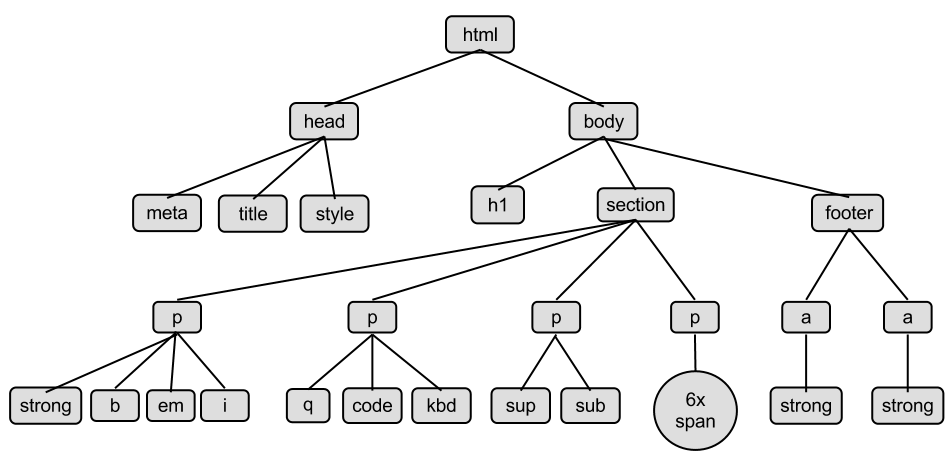
\includegraphics[width=4.5in]{bs-parse-tree.png}
  \caption{Arbol de objetos}
  \label{img:arbol de objetos}
\end{figure}

Este algoritmo, no solo permite el recorrido automático del árbol en busca del texto del documento al
completo, sino que permite además la posibilidad de recorrer el mismo de forma manual, por lo que es posible
acceder a todos los objetos del árbol empleando métodos de navegación como \emph{soup.head, soup.parent,
soup.next\_sibling, ...}.

\subsection{jusText}
\label{subsec:justext}

\textbf{jusText} \cite{justext} es una herramienta para eliminar el contenido repetitivo, como los enlaces
de navegación, encabezados y pies de página de los documentos HTML. Este algoritmo, está diseñado para
preservar el texto que contiene frases completas.

\subsubsection{Preprocesamiento}
\label{subsubsec:preprocesamiento}

Previamente a cualquier fase y con el fin de facilitar el trabajo heurístico, se realiza un preprocesamiento 
del documento HTML. Durante este proceso, se elimina el contenido de ciertas etiquetas como \emph{<header>}, 
\emph{<style>} y \emph{<script>}. Además, el contenido de etiquetas como \emph{<select>} se clasifica 
inmediatamente como contenido basura. Lo mismo ocurre con los bloques que contienen ciertos símbolos 
especiales como el de copyright ©.

\subsubsection{Segmentación}
\label{subsubsec:segmentacion}

Tras una previa fase de preprocesamiento, se procede a lo que se conoce como segmentación. La idea es formar 
bloques de texto dividiendo la página HTML por etiquetas. Una secuencia de dos o más etiquetas como 
\emph{<br>}, \emph{<div>, ...}, separaría los bloques. 

Para la segmentación de bloques, la clave es que los bloques largos y algunos bloques cortos pueden
clasificarse con una confianza muy alta. El resto de bloques cortos pueden clasificarse observando los
bloques circundantes. 

Aunque no sea habitual, puede ocurrir que el contenido de estos bloques no sea homogéneo, es decir, que
dentro de un mismo bloque haya una mezcla de información importante con contenido basura, denominado
\emph{'boilerplate'}. Se resumen a continuación algunos aspectos en relación.

\begin{itemize}
  \item Los bloques cortos que contienen un enlace son casi siempre del tipo \emph{'boilerplate'}.
  \item Los bloques que contienen muchos enlaces son casi siempre del tipo \emph{'boilerplate'}.
  \item Tanto los bloques buenos como los bloques de tipo \emph{'boilerplate'} tienden a crear grupos, es 
  decir, un bloque \emph{'boilerplate'} suele estar rodeado de otros bloques de su mismo tipo y viceversa.
  \item Los bloques largos que contienen texto gramatical forman parte del contenido valioso, mientras que 
  todos los demás bloques largos son casi siempre del tipo \emph{'boilerplate'}.
\end{itemize}

Con respecto al ultimo punto, decidir si un texto es gramatical o no puede ser complicado, \textbf{jusText} 
emplea una simple heurística basada en el volumen de palabras con sentido gramatical. Mientras que un texto 
gramatical suele contener un cierto porcentaje de estas palabras, los contenidos de tipo \emph{'boilerplate'} 
suelen carecer de ellas.

\subsubsection{Clasificación de bloques}
\label{subsubsec:clasificacion de bloques}

Tras la fase de preprocesamiento y segmentación se procede a la clasificación de bloques, donde a cada uno
de estos bloques se le asigna una clase dependiendo de su naturaleza. En el fragmento de código 
\ref{cod:justext - algoritmo de clasificacion} se muestra paso a paso como se determina el tipo de clase 
para cada bloque.

\begin{codefloat}
  \inputencoding{latin1}
  \lstinputlisting[style=CppExample]{scripts/justext-clasificacion.py}
  \inputencoding{utf8}
  \caption{jusText - Algoritmo de clasificación}
  \label{cod:justext - algoritmo de clasificacion}
\end{codefloat}

Analizando el algoritmo, se observa que se definen dos tipos de variables, la densidad y la longitud. 
Mientras que la longitud es el número de caracteres por bloque, la densidad se define como la proporción 
de caracteres o palabras dentro de una etiqueta de tipo \emph{<a>}, o una lista de parada.

Además de los valores de densidad y longitud, el algoritmo toma como parámetros dos enteros definidos como
\emph{LENGTH\_LOW} y \emph{LENGTH\_HIGH}, y también tres números de coma flotante, \emph{MAX\_LINK\_DENSITY},
\emph{STOPWORDS\_LOW} y \emph{STOPWORDS\_HIGH}. Los dos primeros establecen los umbrales para dividir los 
bloques por su longitud. Los dos últimos dividen los bloques por la densidad de palabras de parada en bajos, 
medianos y altos.

Si volvemos a observar el algoritmo \ref{cod:justext - algoritmo de clasificacion}, nos damos cuenta de
que solo se ha realizado una clasificación real sobre los bloques de tamaño medio y largo. En la tabla
\ref{tab:justext - clasificacion de bloques long & medium size} se muestra a modo de resumen como se actúa 
sobre este tipo de bloques.

\begin{table}[h]
  \begin{center}
  \begin{tabular}{| c | c | c |}
  \hline \textbf{Block size} & \textbf{Stopwords density} & \textbf{Class} \\ \hline
  medium size & low & bad \\ \hline
  long & low & bad \\ \hline
  medium size & medium & near-good \\ \hline
  long & medium & near-good \\ \hline
  medium size & high & near-good \\ \hline
  long & high & good \\ \hline
  \end{tabular}
  \caption{jusText - Clasificación de bloques long \& medium size}
  \label{tab:justext - clasificacion de bloques long & medium size}
  \end{center}
\end{table}

\subsubsection{Reclasificación de bloques}
\label{subsubsec:reclasificacion de bloques}

¿Qué ocurre entonces con los bloques cortos y los bloques casi buenos? La reclasificación en este caso se 
realiza en función de los bloques circundantes. Los bloques ya clasificados como buenos o malos sirven 
como piedras base en esta etapa y su clasificación se considera fiable, por lo que nunca se modifica. Esta 
reclasificación se puede ver resumida en la figura \ref{img:justext - reclasificacion de bloques}.

\begin{figure}[tphb]
  \centering
  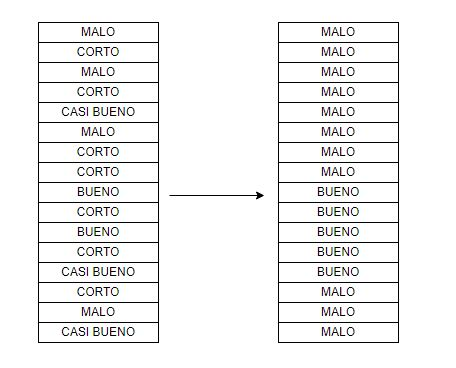
\includegraphics[width=3.6in]{justext-blocks-classification.jpg}
  \caption{jusText - Reclasificación de bloques}
  \label{img:justext - reclasificacion de bloques}
\end{figure}

La idea que subyace a la reclasificación es que los bloques \emph{'boilerplate'} suelen estar rodeados de 
otros bloques \emph{'boilerplate'} y viceversa. Los bloques casi buenos suelen contener datos útiles del 
corpus si se encuentran cerca de bloques buenos. Los bloques cortos suelen ser útiles sólo si están rodeados 
de bloques buenos por ambos lados.

\subsubsection{Bloques de cabecera}
\label{subsubsec:bloques de cabecera}

En cuanto a los bloques de cabecera, aquellos encerrados en etiquetas del tipo \emph{<h1>}, \emph{<h2>}, 
..., son tratados de una manera especial. El objetivo es conservar estos bloques en los textos determinados 
como buenos.

Para el tratamiento especial de bloques de cabecera se añaden dos etapas. La primera etapa, conocida como 
preprocesamiento, se ejecuta justamente después de la clasificación y justo antes de la reclasificación de 
bloques. La segunda etapa, conocida como postprocesamiento, se ejecuta después de la reclasificación.

\begin{enumerate}
  \item Clasificación de bloques.
  \item \textbf{Preprocesamiento de bloques de cabecera}.
  \item Reclasificación de bloques.
  \item \textbf{Postprocesamiento de bloques de cabecera}.
\end{enumerate}

Durante esta fase de preprocesamiento, se buscan bloques de cabecera cortos que precedan a bloques buenos, 
y que al mismo tiempo no haya más caracteres entre el bloque de cabecera y el bloque bueno. El propósito 
de esto es preservar los bloques cortos entre el encabezado y el texto bueno que, de otro modo, podrían 
ser seleccionados como malos durante el proceso de reclasificación.

Por otro lado, en el postprocesamiento, se buscan de nuevo bloques de cabecera que precedan a bloques
buenos, y que al mismo tiempo no haya más caracteres entre el bloque de cabecera y el bloque bueno. El
propósito es que algunas cabeceras cortas y casi buenas puedan clasificarse como buenas si preceden a
bloques buenos que, de otro modo, habrían sido clasificadas como malas tras de la reclasificación.

\subsection{news-please}
\label{subsec:news-please}

Otro \emph{web scraper}, y al mismo tiempo \emph{web crawler}, de código abierto es \textbf{news-please}
\cite{news-please}. Esta biblioteca está desarrollada para cumplir cinco requisitos: extracción de
noticias de cualquier sitio web, extracción completa del sitio web, alta calidad de la información
extraída, facilidad de uso y mantenibilidad.

A diferencia de otras bibliotecas ya mencionadas anteriormente, se emplean herramientas ya existentes las 
cuales se amplían con nuevas funcionalidades con el objetivo de cumplir con los requisitos señalados.

\begin{figure}[tphb]
  \centering
  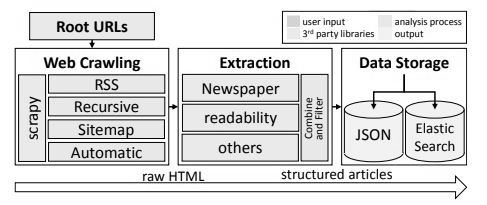
\includegraphics[width=4.5in]{newsplease-processing.jpg}
  \caption{news-please - Proceso de scraping y crawling}
  \label{img:news-please - proceso de scraping y crawling}
\end{figure}

\subsubsection{Web crawling en news-please}
\label{subsubsec:web crawling en news-please}

En cuanto al proceso de \emph{web crawling}, primero se descarga el documento y en segundo lugar, con el 
objetivo de encontrar todos los artículos publicados en dicho documento, se procede con el \emph{crawling}. 
Como se muestra en la figura \ref{img:news-please - proceso de scraping y crawling}, para este proceso se 
dispone de cuatro técnicas diferentes.

La primera técnica se conoce como RSS, en la que se analizan canales RSS con el objetivo de encontrar 
artículos recientes. Un RSS \cite{rss-sitemaps} es un tipo de formato de datos utilizado para proporcionar 
a los usuarios contenidos actualizados con frecuencia.

En segundo lugar, se emplea un seguimiento recursivo de los enlaces internos en las páginas rastreadas.
El uso del \emph{framework} \emph{scrapy} es fundamental independientemente de la técnica.

La tercera técnica consiste en analizar los \emph{sitemaps} en busca de enlaces a todos los artículos. Un 
\emph{sitemap} \cite{rss-sitemaps} es un archivo que enumera las URL's visibles de un determinado sitio, 
cuyo objetivo principal es revelar dónde pueden buscar contenido las máquinas.

Finalmente se prueba con el \emph{crawling} a través de los \emph{sitemaps} y en caso de que se produzca 
cualquier error se vuelve a la técnica de \emph{crawling} recursiva.

Estos cuatro enfoques también pueden combinarse, por ejemplo, iniciando dos instancias en paralelo, una en 
modo automático para obtener todos los artículos publicados hasta el momento y otra instancia en modo RSS 
para recuperar los artículos recientes.

\subsubsection{Web scraping en news-please}
\label{subsubsec:web scraping en news-please}

Para el proceso de \emph{web scraping}, se emplean herramientas ya existentes en el mercado con el objetivo 
de obtener la información deseada, título, contenido principal, autor, fecha... Herramientas como 
\textbf{Newspaper3k} \ref{subsec:newspaper3k} o \textbf{Readability} \ref{subsec:readability} son utilizadas 
para este proceso de extracción.

\begin{codefloat}
  \inputencoding{latin1}
  \lstinputlisting[style=CppExample, showstringspaces=false]{scripts/newsplease-scrape.py}
  \inputencoding{utf8}
  \caption{news-please - Extracción de contenido relevante}
  \label{cod:news-please - extraccion de contenido relevante}
\end{codefloat}

Una vez que el contenido relevante ha sido extraído, se almacena de forma estructurada en determinados
archivos de forma que este pueda ser consultado posteriormente.

\subsection{Libextract}
\label{subsec:libextract}

\textbf{Libextract} \cite{libextract} es una biblioteca de extracción de datos con capacidad estadística
que funciona con documentos HTML y XML escrita en Python. En cuanto al algoritmo de extracción empleado,
\textbf{eatiht}, funciona en base a una simple suposición en la cual los datos aparecen como colecciones 
de elementos repetitivos.

\subsubsection{eatiht como algoritmo de partición}
\label{subsubsec:eatiht como algoritmo de particion}

\textbf{eatiht} \cite{eatiht} es una posible solución en una línea de muchas soluciones imperfectas a uno 
o más problemas en algún subcampo de la extracción de datos. En pocas palabras, este algoritmo intenta 
extraer el texto central de un sitio web determinado.

Se trabaja con dos supuestos, en primer lugar se determina que el texto considerado como valioso es largo, 
mientras que los textos 'basura' suelen disponer de una menor cantidad de información. Por otro lado, se 
determina que los textos de valor vienen agrupados.

Imaginemos un documento HTML sencillo en el que aplicando una determinada expresión XPath como la siguiente,
\emph{/text()[string-length(normalize-space()) > 20]}, se seleccionen todos los nodos de texto que tengan 
una longitud de cadena superior a veinte.

\begin{Schunk}
  \begin{Soutput}
    /html/body/div/article
    /html/body/div/div
    /html/body/div/footer
  \end{Soutput}
\end{Schunk}

Dada una posible solución como la anterior, se debe contar el numero de nodos hijo de cada uno con el 
objetivo de crear una distribución de frecuencias de cada conjunto a través de un histograma.

\begin{Schunk}
  \begin{Soutput}
    /html/body/div/article   | — — — —
    /html/body/div/div       | —
    /html/body/div/footer    | —
  \end{Soutput}
\end{Schunk}

Tras este proceso y con una simple comprensión de la lista de conjuntos, es posible adquirir algunos, pero 
no todos los nodos de texto que existen en el subárbol deseado. Veamos el funcionamiento de dicho algoritmo.

\begin{codefloat}
  \inputencoding{latin1}
  \lstinputlisting[style=CppExample, showstringspaces=false]{scripts/libextract-eatiht.py}
  \inputencoding{utf8}
  \caption{Libextract - Funcionamiento de eatiht}
  \label{cod:libextract - funcionamiento de eatiht}
\end{codefloat}

\subsection{html\_text}
\label{subsec:html_text}

\textbf{html\_text} \cite{html-text} es una biblioteca de Python encargada de convertir un documento HTML
en texto plano. Las principales diferencias frente a algoritmos como \textbf{Beautiful Soup},
\ref{subsec:beautiful soup} donde se emplean expresiones del tipo \emph{.get\_text()}, o frente a expresiones
XPath como \emph{.xpath('//text()')}, son las siguientes:

\begin{enumerate}
  \item El texto extraído en este caso, no contiene código JavaScript del propio documento, así como 
  comentarios o cualquier contenido que no sea visible por el usuario.
  \item La normalización de espacios también se tiene en cuenta, pero de una manera más inteligente que
  con el uso simple de expresiones XPath, \emph{.xpath('normalize-space())}, ya que añade espacios alrededor
  de los elementos en línea, y evitar añadir espacios extra para la puntuación.
  \item Se añaden nuevas líneas de forma frecuente, por ejemplo después de los encabezados o párrafos, para 
  que el texto de salida se parezca más a cómo se presenta en los navegadores.
\end{enumerate}

En cuanto a la heurística, en primer lugar se limpia el documento empleando como instancia
\emph{lxml.html.clean.Cleaner}, y después, se procede con la conversión de árbol de objetos a texto,
empleando para ello lo que se conoce como \emph{'chunks'}.

\subsubsection{Normalización de espacio}
\label{subsubsec:normalizacion de espacio}

El uso habitual del algoritmo se consigue ejecutando la función de extracción de texto principal, de forma 
que un documento HTML se pasa por parámetro y se devuelve como salida la parte de información que se determina
como valiosa.

\begin{Schunk}
  \begin{Soutput}
    >>> html_text.extract_text('<h1>Hello</h1> world!')
    # 'Hello\n\nworld!'
  \end{Soutput}
\end{Schunk}

En cuanto a la estructura del texto extraído, es posible personalizar cómo se añaden nuevas líneas al mismo
utilizando los argumentos \emph{newline\_tags} y \emph{double\_newline\_tags}. De esta forma el algoritmo 
es capaz de distinguir de forma automática aquellas secciones del documento que deben ser separadas por 
línea simple o por doble línea.

\begin{Schunk}
  \begin{Soutput}
    NEWLINE_TAGS = frozenset([
      'article', 'aside', 'br', 'dd', 'details', 'div', 'dt', 'fieldset',
      'figcaption', 'footer', 'form', 'header', 'hr', 'legend', ...
    ])

    DOUBLE_NEWLINE_TAGS = frozenset([
      'blockquote', 'dl', 'figure', 'h1', 'h2', 'h3', 'h4', 'h5', 'h6', 'ol',
      'p', 'pre', 'title', 'ul'
    ])
  \end{Soutput}
\end{Schunk}

Imaginemos que se desea ejecutar \textbf{html\_text} sobre un documento HTML como el siguiente
\emph{<div>Hello</div> world!}, donde el texto principal esta separado por una etiqueta de tipo \emph{<div>}.
A partir de la gestión de espacio según el tipo de etiqueta, se determina la solución obtenida.

\begin{Schunk}
  \begin{Soutput}
    >>> newline_tags = html_text.NEWLINE_TAGS - {'div'}
    >>> html_text.extract_text('<div>Hello</div> world!',
    ...                        newline_tags=newline_tags)
    # 'Hello world!'
  \end{Soutput}
\end{Schunk}

\subsection{html2text}
\label{subsec:html2text}

\textbf{html2ext} \cite{html2text} es un script de Python que convierte un documento HTML a texto ASCII, 
el cual también resulta ser un formato de texto válido a HTML. Imaginemos que se dispone de un documento 
HTML sencillo como el siguiente, \emph{'<p><strong>Zed's</strong> dead baby, <em>Zed's</em> dead.</p>'}, 
veamos la salida obtenida:

\begin{Schunk}
  \begin{Soutput}
    >>> html2text("<p><strong>Zed's</strong> dead baby, <em>Zed's</em> dead.</p>"))
    # **Zed's** dead baby, _Zed's_ dead.
  \end{Soutput}
\end{Schunk}

Si por el contrario se desea que la solución sea limpia, es posible eliminar todos los caracteres de
marcado del texto obtenido empleando la función \emph{handle} como método de extracción.

\begin{Schunk}
  \begin{Soutput}
    >>> handle("<p><strong>Zed's</strong> dead baby, <em>Zed's</em> dead.</p>"))
    # Zed's dead baby, Zed's dead.
  \end{Soutput}
\end{Schunk}

En cuanto a la heurística de extracción, el algoritmo simplemente analiza el documento a través de
\emph{html.parser}, y a continuación envuelven todos los párrafos del texto proporcionado.

\subsection{Readability}
\label{subsec:readability}

Dado un documento HTML, \textbf{Readability} \cite{readability} extrae el cuerpo del texto principal del 
mismo. Previamente a la extracción de texto se produce una limpieza, donde se eliminan \emph{tags} y 
atributos del propio documento. Este preprocesamiento se lleva a cabo mediante el uso de expresiones 
regulares.

\subsubsection{Heurística de nodo candidato}
\label{subsubsec:heuristica de nodo candidato}

La heurística de esta biblioteca es similar a la empleada por \textbf{Goose3} \ref{subsec:goose3} para
calcular el mejor nodo del árbol. A partir de una puntuación dada para cada nodo se determina aquel cuya
puntuación se máxima con el objetivo de obtener el nodo con una mayor cantidad de información.

\begin{codefloat}
  \inputencoding{latin1}
  \lstinputlisting[style=CppExample, showstringspaces=false]{scripts/readability-menjor-candidato.py}
  \inputencoding{utf8}
  \caption{Readability - Selección del nodo candidato}
  \label{cod:readability - seleccion del nodo candidato}
\end{codefloat}

Una vez seleccionado dicho nodo, se busca en nodos hermanos con el objetivo de encontrar aquellos cuya
información esté relacionada con el mismo, y, por tanto, sean de valor.

\subsection{Trafilatura}
\label{subsec:trafilatura}

Al igual que muchas otras, \textbf{Trafilatura} \cite{trafilatura} es una herramienta de búsqueda de texto
en la web que descarga, analiza y extrae datos de documentos HTML. El algoritmo de extracción no solo se
centra en los metadatos, el cuerpo del texto o comentarios, también trata de conservar parte del formato
y la estructura de la página.

En cuanto a la heurística, esta se fundamenta en una cascada de filtros determinados por una serie de 
reglas y metodología del contenido. En las siguientes secciones se determinan los pasos que realiza el
algoritmo para una extracción exitosa.

\subsubsection{Delimitación de contenido}
\label{subsubsec:delimitacion de contenido}

El objetivo de esta primera fase es separar el contenido con valor del contenido basura o
\emph{'boilerplate'}. Para ello el algoritmo hace uso de expresiones XPath dirigidas tanto a atributos HTML,
como al contenido principal del documento.

\begin{Schunk}
  \begin{Soutput}
    DISCARD_XPATH = [
      '''.//*[(self::div or self::item or self::list or self::p or self...)][
      contains(@id, "related") or contains(@class, "nav") or 
      contains(@class, "subnav") or contains(@id, "cookie") or ...]'''
    ]
  \end{Soutput}
\end{Schunk}

Inicialmente, el uso de expresiones como las mostradas se emplea para excluir partes o secciones no deseadas 
del código HTML, por ejemplo la expresión \emph{<div class='nav'>} eliminaría todo el contenido que incluyese
cualquier etiqueta \emph{<div>} de tipo \emph{'navigation'}.

Tras esta exclusión de contenido \emph{'boilerplate'}, el algoritmo se centra nuevamente en el uso de 
expresiones XPath, pero en este caso que abarquen todo el contenido de valor a extraer. Expresiones como
\emph{<section id='entry-content'>} o como las mostradas a continuación, buscan partes de contenido
potencialmente valioso.

\begin{Schunk}
  \begin{Soutput}
    BODY_XPATH = [
      '''.//*[(self::article or self::div or self::main or self::section)][
      contains(@id, "content-main") or
      contains(@class, "entry-content") or 
      contains(@class, "content-main") or ...]'''
    ]
  \end{Soutput}
\end{Schunk}

Las mismas operaciones se realizan para los comentarios en caso de que estos formen parte de la extracción. 
Los nodos seleccionados del árbol HTML se procesan, es decir, se comprueba su relevancia y se simplifican 
en cuanto a su estructura HTML.

\begin{Schunk}
  \begin{Soutput}
    COMMENTS_XPATH = [
      '''.//*[(self::div or self::section or self::list)][
      contains(@id, 'commentlist') or 
      contains(@class, 'commentlist') or 
      contains(@class, 'comment-page') or ...]'''
    ]
  \end{Soutput}
\end{Schunk}

\subsubsection{Algoritmos de respaldo}
\label{subsubsec:algoritmos de respaldo}

Si se detecta que la extracción realizada ha sido defectuosa, se ejecuta lo que se conocen como algoritmos 
de respaldo. Estos algoritmos aplican una heurística basada en la longitud de las líneas, la relación 
texto/marcado y la posición/profundidad de los elementos en el árbol HTML.

\begin{codefloat}
  \inputencoding{latin1}
  \lstinputlisting[style=CppExample, showstringspaces=false]{scripts/trafilatura-respaldo1.py}
  \inputencoding{utf8}
  \caption{Trafilatura - Readability como algoritmo de respaldo}
  \label{cod:trafilatura - readability como algoritmo de respaldo}
\end{codefloat}

Esta fase de la extracción combina dos bibliotecas para su funcionamiento, tanto \textbf{Readability}
\ref{subsec:readability} como \textbf{jusText} \ref{subsec:justext} se encargan de servir como redes de
seguridad y \emph{fallbacks} en caso de que la extracción anterior resultase errónea. Se muestra el código 
fuente de ambos en \ref{cod:trafilatura - readability como algoritmo de respaldo} y 
\ref{cod:trafilatura - justext como algoritmo de respaldo}.

\begin{codefloat}
  \inputencoding{latin1}
  \lstinputlisting[style=CppExample, showstringspaces=false]{scripts/trafilatura-respaldo2.py}
  \inputencoding{utf8}
  \caption{Trafilatura - jusText como algoritmo de respaldo}
  \label{cod:trafilatura - justext como algoritmo de respaldo}
\end{codefloat}

Una vez aplicados estos algoritmos, su resultado se compara con la extracción inicial con el objetivo de 
determinar cual es la más eficaz en términos de longitud e impurezas.

\subsubsection{Extracción base}
\label{subsubsec:extraccion base}

En caso de que ni la delimitación de contenido, ni los algoritmos de respaldo funcionen, se ejecuta una
extracción base para buscar elementos de texto \emph{'salvajes'} que probablemente se hayan pasado por alto.
Esto implica descartar las partes no deseadas, y buscar cualquier elemento que pueda contener contenido
textual útil, por ejemplo elementos \emph{<div>} sin párrafos.

Como resultado de toda esta consecución de algoritmos se obtienen los textos principales y los potenciales
comentarios de los documentos HTML analizados, con la posibilidad de conservar elementos estructurales como
párrafos, títulos, listas, comillas o saltos de línea. En la extracción, también se incluyen metadatos, 
es decir, título, nombre del sitio, autor, fecha, categorías y etiquetas del propio documento.

\subsection{Dragnet}
\label{subsec:dragnet}

\textbf{Dragnet} \cite{dragnet} es una biblioteca de \emph{web scraping} escrita en Python, la cual empleando 
inteligencia artificial es capaz de extraer el texto principal de documento HTML.

Algoritmos de extracción ya mostrados, como \textbf{inscriptis} \ref{subsec:inscriptis}, trabajan dividiendo 
el documento HTML en una secuencia de bloques que posteriormente son clasificados empleando la densidad de 
los mismos como instrumento de medida. \textbf{Dragnet} combina esta clasificación de bloques con el 
aprendizaje automático para minimizar el contenido basura y maximizar la obtención de información valiosa.

\subsubsection{Extracción enfocada al aprendizaje automatico}
\label{subsubsec:extraccion enfocada al aprendizaje automatico}

El algoritmo comienza dividiendo el documento en una secuencia de bloques, utilizando el DOM \footnote{El 
DOM define la manera en que objetos y elementos se relacionan entre sí en el navegador y en el documento.} 
y un conjunto específico de etiquetas como \emph{<div>}, \emph{<p>} o \emph{<h1>}, que modifican la 
estructura del propio documento. Para crear esta secuencia de bloques el algoritmo itera por el DOM, y cada 
vez que se encuentra cierto tipo de etiqueta se crea un nuevo bloque.

Una vez dividido el documento en bloques, se asocia un token con cada bloque del mismo. Estos tokens serán 
útiles en un clasificador para separar el contenido con valor del contenido \emph{'boilerplate'} a nivel 
de bloque. Cualquier bloque con más del 10\% de los tokens extraídos se etiqueta como contenido valioso.

\subsubsection{Características del modelo}
\label{subsubsec:carcateristicas del modelo}

Además de la división por bloques y del aprendizaje automático, esta biblioteca introduce una serie de 
características diseñadas heurísticamente para capturar información semántica en el código HTML que dejan
los programadores. 

En primer lugar, muchos atributos como \emph{id} o \emph{class}, y etiquetas HTML incluyen tokens de tipo 
\emph{comment}, \emph{header} y \emph{nav}. Estos nombres descriptivos son utilizados por los desarrolladores 
cuando programan código en CSS y JavaScript y, puesto que se eligen con el objetivo de que tengan sentido 
para el programador, incorporan cierta información semántica sobre el contenido del bloque.

\begin{Schunk}
  \begin{Soutput}
    attribute_tokens = (
      ('id',
        ('nav', 'ss', 'top', 'content', 'link', 'title', 'comment',...)),
      ('class',
        ('menu', 'widget', 'nav', 'share', 'facebook', 'cat', 'top', 'content',
        'item', 'twitter', 'button', 'title', 'header', 'ss', 'post', ...))
    )
  \end{Soutput}
\end{Schunk}

Otro conjunto de características se corresponde con la densidad de texto y densidad de enlaces. La intuición 
es que los bloques de contenido tienen una mayor densidad de texto y una menor densidad de enlaces que los 
bloques denominados \emph{'boilerplate'}, ya que muchos de estos últimos son bloques que consisten en breves
fragmentos de palabras o son principalmente texto ancla.

Por último, la tercera característica incluye varias ideas, por un lado, la relación entre la longitud del
texto y el número de etiquetas HTML, y en segundo lugar la agrupación de bloques \emph{'boilerplate'}. La 
idea final es combinar la proporción de etiquetas de contenido valioso y la proporción de etiquetas de 
contenido basura en un enfoque de agrupación de \emph{k-means} no supervisado, de modo que los bloques sin 
contenido se agrupen naturalmente cerca del origen.

\subsection{Goose3}
\label{subsec:goose3}

Otra biblioteca de programación cuyo objetivo es la extracción de texto en artículos es \textbf{Goose} 
\cite{goose3}. Inicialmente, el proyecto fue desarrollado en Java, pero a lo largo del tiempo han ido 
surgiendo nuevas versiones en diferentes lenguajes de programación como Scala o Python.

El objetivo del software es tomar cualquier documento de noticias o página web de tipo artículo y además
del cuerpo principal, extraer la imagen, videos, descripción y meta tags del mismo.

\subsubsection{Cálculo del mejor nodo}
\label{subsubsec:calculo del mejor nodo}

La técnica que emplea esta biblioteca para la extracción de contenido principal es muy similar a la que 
se emplea en muchos otros algoritmos de extracción, donde un árbol se recorre con el fin de obtener la 
mayor cantidad de información posible.

El primer paso consiste en recorrer todo los posibles nodos del árbol para almacenar aquellos que posean 
texto legible. En el fragmento de código \ref{cod:goose3 - calculo del mejor nodo 1} se muestra una primera 
parte de como Goose realiza dicho recorrido.

\begin{codefloat}
  \inputencoding{latin1}
  \lstinputlisting[style=CppExample, showstringspaces=false]{scripts/goose3-extraccion1.py}
  \inputencoding{utf8}
  \caption{Goose3 - Cálculo del mejor nodo 1}
  \label{cod:goose3 - calculo del mejor nodo 1}
\end{codefloat}

Una vez los nodos han sido almacenados, se determina una puntuación para cada uno de ellos. Esta puntuación 
se calcula en función del número de palabras con sentido gramatical del texto contenido en cada nodo, más
una cierta cantidad denominada \emph{'boost-score'}. 

\begin{Schunk}
  \begin{Soutput}
    upscore = int(word_stats.get_stopword_count() + boost_score)
  \end{Soutput}
\end{Schunk}

Una vez determinada la puntuación de cada nodo se procede de la manera mostrada en 
\ref{cod:goose3 - calculo del mejor nodo 2} donde se compara la puntuación de cada nodo, con el objetivo 
de encontrar aquel cuya puntuación sea máxima.

\begin{codefloat}
  \inputencoding{latin1}
  \lstinputlisting[style=CppExample, showstringspaces=false]{scripts/goose3-extraccion2.py}
  \inputencoding{utf8}
  \caption{Goose3 - Cálculo del mejor nodo 2}
  \label{cod:goose3 - calculo del mejor nodo 2}
\end{codefloat}

\subsection{Newspaper3k}
\label{subsec:newspaper3k}

Inspirada en otras bibliotecas de HTTP e impulsada por el analizador \emph{lxml}, \textbf{Newspaper3k}
\cite{newspaper3k} es una biblioteca de Python encargada de realizar minado en la web. Entre muchas de las
características que hacen destacar esta biblioteca sobre el resto se puede destacar las siguientes:

\begin{itemize}
  \item Capacidad de descarga de artículos en paralelo gracias al uso de multiples hilos.
  \item Identificación de URL's de artículos.
  \item Extracción de texto de un documento HTML.
  \item Extracción de imágenes de un documento HTML.
  \item Extracción de palabras clave de un texto.
  \item Resumen del contenido de un documento texto.
  \item Extracción de términos de tendencia de Google.
  \item Trabajo con multiples idiomas.
\end{itemize}

En cuanto a la heurística de extracción, se usa gran parte del código fuente de \textbf{Goose} 
\ref{subsec:goose3}, por lo que la fuente de cálculo del mejor nodo, así como al selección del mismo a 
través del número de palabras clave será esencial en este caso también.

\subsubsection{Heurística según el idioma}
\label{subsubsec:heuristica segun el idioma}

Uno de los aspectos importantes del algoritmo de extracción de texto gira en torno al recuento del número 
de palabras clave o palabras con sentido gramatical presentes en un texto. Estas palabras son algunas de 
las palabras funcionales cortas más comunes de un idioma, como \emph{the, is, at, which, on}... 

Al trabajar con múltiples idiomas, esta heurística debe cambiar, puesto que distintos tipos de palabras
aparecen para cada uno. Para idiomas latinos, se proporciona una lista de palabras clave en formato 
\emph{stopwords-<código de idioma>}. A continuación, se toma un texto de entrada y se convierte en palabras 
dividiendo los espacios en blanco, para más tarde realizar un conteo y enumerar la cantidad de palabras 
clave.

Para los idiomas no latinos, es necesario dividir las palabras en tokens de una manera diferente, puesto
que la división por espacios en blanco no funciona para idiomas como el chino o el árabe. Para el idioma
chino se emplea una nueva biblioteca de código abierto llamada \emph{jieba}, sin embargo, para el árabe
se utiliza un tokenizador especial, \emph{nltk} que se encarga de hacer el mismo trabajo como se muestra 
en el fragmento de código \ref{cod:newspaper3k - heuristica en el arabe}.

\begin{codefloat}
  \inputencoding{latin1}
  \lstinputlisting[style=CppExample, showstringspaces=false]{scripts/newspaper3k-stopword.py}
  \inputencoding{utf8}
  \caption{Newspaper3k - Heurística en el árabe}
  \label{cod:newspaper3k - heuristica en el arabe}
\end{codefloat}

\subsection{BoilerPy3/BoilerpipeR}
\label{subsec:boilerpy/boilerpiper}

\textbf{BoilerpipeR} \cite{boilerpipeR-cran} en R, y \textbf{BoilerPy3} \cite{boilerpy} en Python, son 
paquetes que proporcionan una interfaz para una biblioteca Java. Soportan la extracción genérica del 
contenido del texto principal de los archivos HTML y, por tanto, elimina los anuncios, las barras laterales 
y cabeceras del contenido fuente HTML.

En cuanto a la heurística, el algoritmo original se basa en separar el contenido boilerplate del contenido
valioso. Para ello se emplean algoritmos de apoyo con el fin de detectar y eliminar el exceso de desorden
alrededor del contenido principal de una página web.

\subsubsection{Multiplicidad de extractores}
\label{subsubsec:multiplicidad de extractores}

El paquete dispone de varios extractores para diferentes situación de extracción, con múltiples heurísticas
las cuales se especifican a continuación. Por otro lado, cada extractor es capaz de manejar las excepciones 
que se produzcan durante la extracción y devolver cualquier texto que haya sido extraído con éxito.

\begin{itemize}
  \item DefaultExtractor: extractor muy simple, sin heurística, bastante genérico pero completo.
  \item ArticleExtractor: gestiona los artículos de noticias. Funciona muy bien para la mayoría de los 
  tipos de HTML tipo artículo.
  \item ArticleSentencesExtractor: se encarga de la extracción de frases en artículos de prensa.
  \item LargestContentExtractor: se centra en extraer el componente de texto más grande de una página. 
  \item CanolaExtractor: : extractor de texto entrenado en un \emph{krdwrd}.
  \item KeepEverythingExtractor: marca todo como contenido, debería devolver el texto de entrada. Se emplea 
  en caso de error, para comprobar si el error procede de un extractor en particular o de otro lugar.
  \item NumWordsRulesExtractor: se basa únicamente en el número de palabras por bloque.
\end{itemize}

\section{Paquetes de R encontrados durante el proceso de búsqueda}
\label{sec:paquetes de r encontrados durante el proceso de busqueda}

Además de la introducción de aquellas bibliotecas de Python destinadas al \emph{web scraping}, se incluye 
en la evaluación paquetes con la misma funcionalidad desarrollados en R. Por ello, se realizará una 
sinopsis de aquellos paquetes de R que realicen \emph{web scraping} y puedan ser incluidos en el proceso 
de evaluación.

\begin{table}[h]
  \begin{center}
  \begin{tabular}{| c | c | c | c | c | c |} \hline 
    \textbf{rvest} & \textbf{rcrawler} & \textbf{htm2txt} & \textbf{rselenium} & \textbf{scraper} & \textbf{boilerpiper} \\ \hline
    xml2 & xml2 & N/A & XML & XML & XML \\ \hline
  \end{tabular}
  \caption{Emparejamientos paquete-analizador}
  \label{tab:emparejamientos paquete-analizador}
  \end{center}
\end{table}

Antes de comenzar con la sinopsis de paquetes, es conveniente revisar el apéndice \ref{cha:analizadores 
empleados en los paquetes de web scraping}, donde se realiza una breve introducción de aquellos analizadores 
empleados en los mismos. Los ’emparejamientos’ entre paquete-analizador se recogen en la tabla 
\ref{tab:emparejamientos paquete-analizador} a modo de resumen.

Se puede observar que \textbf{htm2txt} no emplea ningún tipo de analizador. En contrapartida hace uso de 
expresiones regulares para eliminar las etiquetas html.

\subsection{rvest}
\label{subsec:rvest}

Inspirada en otras bibliotecas como \textbf{Beautiful Soup} \ref{subsec:beautiful soup}, \textbf{rvest} 
\cite{rvest-cran} es una de las herramientas mas comunes de minado web. Este paquete esta diseñado para 
trabajar con \emph{magrittr}, para facilitar tareas comunes del \emph{web scraping}, y con \emph{polite}, 
para garantizar que se respete el archivo \emph{robots.txt} y no saturar el sitio web con multiples 
peticiones.

En el apéndice \ref{cha:funcionamiento basico de un web scraper} se puede comprobar el funcionamiento del
paquete durante la extracción de parte de un documento HTML. Ademas, se observa que el paquete actúa como 
\emph{wrapper} entre los paquetes \emph{xml2} y \emph{httr}, facilitando así la descarga y manipulación 
de un fichero HTML.

\subsubsection{Elementos a nivel de bloque vs elementos en línea}
\label{subsubsec:elementos a nivel de bloque vs elementos en linea}

El objetivo de \textbf{rvest} es que a partir de una determinada entrada, ya sea una URL o un documento
HTML, extraer el texto principal emulando a un navegador con el fín de que el texto extraído se acerque 
lo máximo posible a la realidad. Para ello el algoritmo se basa en lo que se conoce como elementos a nivel 
de bloque.

Los elementos de un documento HTML se clasifican como elementos de nivel de bloque o de nivel de línea. Un 
elemento de nivel de bloque ocupa todo el espacio horizontal de su contenedor, y un espacio vertical igual 
a la altura de su contenido, creando así lo que se conoce como bloque. Se muestra un ejemplo a continuación.

\begin{Schunk}
  \begin{Soutput}
    <p>This paragraph is a block-level element; its background has been 
    colored to display the paragraph's container element.</p>
  \end{Soutput}
\end{Schunk}

\begin{figure}[tphb]
  \centering
  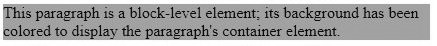
\includegraphics[width=4.5in]{rvest-block-elements.jpg}
  \caption{rvest - Elementos a nivel de bloque}
  \label{img:rvest - elementos a nivel de bloque}
\end{figure}

Los elementos de nivel de bloque pueden contener elementos en línea y otros elementos de nivel de bloque. 
Esta distinción estructural lleva implícita la idea de que los elementos de bloque crean estructuras más 
grandes que los elementos en línea. Ademas, los elementos de nivel de bloque comienzan en líneas nuevas, 
pero los elementos en línea pueden empezar en cualquier parte de una línea. Los elementos que \textbf{rvest}
determina a nivel de bloque son los siguientes:

\begin{Schunk}
  \begin{Soutput}
    block_tag <- c( "address", "article", "aside", "blockquote", "details", 
      "dialog", "dd", "div", "dl", "dt", "fieldset", "figcaption", "figure", 
      "footer", "form", "h1", "h2", "h3", "h4", "h5", "h6", "header", ...")
  \end{Soutput}
\end{Schunk}

\subsection{Rcrawler}
\label{subsec:rcrawler}

\textbf{Rcrawler} \cite{rcrawler-cran} tiene como objetivo el rastreo y la extracción de datos estructurados
de forma paralela. Está diseñado para rastrear, parsear y almacenar páginas web para producir datos que
puede ser utilizados con posterioridad para aplicaciones de análisis.

Entre las características de \textbf{RCrawler} se destaca, el rastreo multihilo, la extracción de contenidos
y la detección de contenidos duplicados. Además, incluye funcionalidades como el filtrado de URL's y tipos
de contenido, el control del nivel de profundidad y un analizador de \emph{robot.txt}.

La principal diferencia entre \textbf{Rcrawler} y otros paquetes de \emph{web scraping} como \textbf{rvest},
es que mientras \textbf{rvest} extrae datos de un documento HTML navegando a través de selectores,
\textbf{Rcrawler} recorre, analiza y extrae todos los datos de todas las páginas web con un solo comando.

\subsubsection{Arquitectura y proceso de extracción en Rcrawler}
\label{subsubsec:arquitectura y proceso de extraccion en rcrawler}

Inspirado en otros paquetes como \textbf{Mercator} o \textbf{Ubicrawler}, y con el objetivo evitar una
sobrecarga del entorno, la arquitectura de \textbf{Rcrawler} es lo más óptima y simple posible. En la
figura \ref{img:rcrawler - arquitectura y componentes principales de rcrawler} se muestra la propia
arquitectura de la herramienta \cite{rcrawler}.

\begin{figure}[tphb]
  \centering
  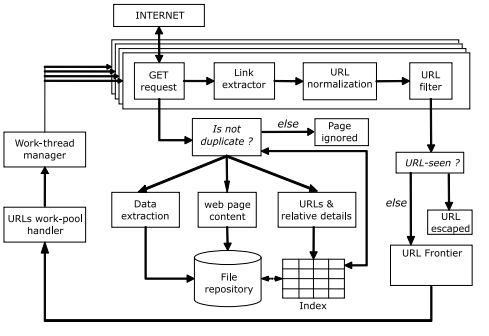
\includegraphics[width=4.5in]{rcrawler-arquitecture.jpg}
  \caption{Rcrawler - Arquitectura y componentes principales de Rcrawler}
  \label{img:rcrawler - arquitectura y componentes principales de rcrawler}
\end{figure}

En primer lugar, el rastreador pone en marcha el entorno de trabajo, es decir, la estructura del índice, 
el repositorio de documentos web y los nodos del clúster para la computación en paralelo. Una vez puesto 
en marcha el entorno de trabajo, se procede con el rastreo el cual es realizado por múltiples hilos de 
trabajo. Por otro lado, el componente \emph{work-pool-handler} prepara un \emph{pool} de URL's para procesar 
en paralelo, donde cada nodo ejecuta las siguientes funciones para cada URL:

\begin{enumerate}
  \item Descargar el documento correspondiente y su cabecera HTTP mediante una petición GET.
  \item Analizar y extraer todos los enlaces contenidos en el documento.
  \item Proceder a la canonización y normalización de URL's.
  \item Aplicar un filtro de URL's, manteniendo sólo aquellas que coincidan con la configuración 
  proporcionada por el usuario, el tipo de archivo y las URL's específicas del dominio.
\end{enumerate}

Tras la descarga del documento a través de la petición GET, se determina si este ya ha sido analizado 
previamente. En caso de que el documento no esté duplicado se procede con el rastreo y la extracción de
datos, con el objetivo de indexar y almacenar los documentos encontrados.

Como resultado, para cada URL cada nodo devuelve su documento HTML, los detalles de la cabecera HTTP y la 
lista de enlaces externos descubiertos. La función \emph{URL-seen} comprueba si la URL ya ha sido procesada.

\subsection{htm2txt}
\label{subsec:htm2txt}

Otro de los paquetes propios de R que se encargan de realizar \emph{web scraping} es \textbf{htm2txt} 
\cite{htm2txt-cran}. Convierte un documento html en textos simples eliminando todas las etiquetas html. 
Este paquete utiliza expresiones regulares para eliminar las etiquetas html. También ofrece las funciones 
\emph{gettxt()} y \emph{browse()}, que permiten obtener o navegar por los textos de una determinada página 
web.

El uso de estas expresiones regulares se hacen notar durante la limpieza del texto extraído, donde la
función \emph{gsub} toma una notable relevancia. Una vez el texto ha sido 'limpiado' se retorna el mismo.

\subsection{scrapeR}
\label{subsec:scraper}

\textbf{scrapeR} \cite{scraper-cran} es otro paquete software que pretende hacer \emph{web scraping} sobre 
documentos basados en la web. El paquete en sí es bastante simple, pues consta de una única función 
encargada de la obtención y creación del árbol DOM para su posterior iteración.

Puesto que no dispone de funciones propias de recorrido del DOM, \textbf{scrapeR} recurre a funciones y
métodos del paquete \emph{XML} para realizar su labor. Esto tiene una ventaja significativa, y es que
permite ejecutar la petición de varias URL's de forma paralela.

\subsection{RSelenium}
\label{subsec:rselenium}

\textbf{RSelenium} \cite{rselenium-cran} es un paquete que tiene como objetivo facilitar la conexión a un 
servidor de Selenium. Además de \emph{web scraping}, \textbf{RSelenium} también permite hacer pruebas de 
unidad y de regresión en las aplicaciones web que se desarrollen utilizando un gran rango de navegadores 
y de sistemas operativos \cite{tfg-daniel-francisco-lopez}. Gracias a esto permite realizar entre otras 
las siguientes tareas:

\begin{enumerate}
  \item Navegar a través de cualquier documento HTML.
  \item Acceder a los elementos del DOM utilizando selectores de id, de clase, de nombre de etiqueta, 
  selectores XPath o CSS.
  \item Enviar eventos de teclado y de ratón a los elementos de la página que se determinen.
  \item Inyectar JavaScript en la página.
  \item Utilizar marcos y ventanas diferenciadas.
\end{enumerate}

A modo de anécdota, cabe destacar que mediante el uso de \textbf{RSelenium} es posible automatizar los
navegadores tanto de forma local como remota. Permite manejar un navegador web nativamente como lo haría
un usuario, lo que supone un salto adelante en términos de automatización del \emph{web scraping}.

\section{Paquetes descartados para el proceso de evaluación}
\label{sec:paquetes descartados para el proceso de evaluacion}

A lo largo de las secciones \ref{sec:bibliotecas de python encontradas durante el proceso de busqueda} y
\ref{sec:paquetes de r encontrados durante el proceso de busqueda} se han introducido y desarrollado
aquellas herramientas de \emph{web scraping} más comunes en el entorno de programación. Con el punto de 
mira en los siguientes capítulos, se pretende enumerar aquellos paquetes descartados para el proceso de 
evaluación.

Ya sea por la simpleza de su heurística, por la similitud con otras herramientas, o por la dificultad en 
la instalación y uso de las mismas, las bibliotecas seleccionadas para el descarte son las siguientes:

\begin{itemize}
  \item \textbf{Dragnet}: Uno de los principales motivos por el que Dragnet a sido descartado es por su 
  complejidad en la instalación. La necesidad de un Docker hace que la mayoría de usuarios no programadores 
  hagan uso de otras herramientas en su lugar.
  \item \textbf{news-please}: El descarte de \textbf{news-please} tiene que ver con el uso de otras
  herramientas para el proceso de \emph{web scraping}. La ausencia de heurística propia y el empleo de otros 
  algoritmos como \textbf{Readability} hace que la evaluación de \textbf{news-please} no tenga sentido.
  \item \textbf{Libextract}: Durante el desarrollo de la herramienta de evaluación, se ha detectado que en
  este caso no se cumplían los requisitos mínimos para la misma. La extracción resultaba errónea para
  ciertos documentos HTML.
  \item \textbf{Newspaper3k}: Tal y como se ha indicado en la sinopsis, el algoritmo emplea gran parte de
  la heurística de \textbf{Goose3} para la extracción de contenido. A falta de heurística propia no tendría
  sentido realizar una evolución del mismo.
  \item \textbf{scrapeR}: La sencillez de la herramienta, y su falta de heurística hace que el descarte 
  de la misma sea necesario. Su única función necesita herramientas XPath para la búsqueda de información
  a través del DOM.
  \item \textbf{RSelenium}: Ademas del necesario emplea de un Docker para su uso, al igual que 
  \textbf{scrapeR}, \textbf{RSelenium} carece de heurística propia, ya que para la extracción de texto 
  emplea expresiones XPath y selectores CSS únicamente.
\end{itemize}

Por último, es notable la falta de algoritmos de R en la herramienta de evaluación. Durante el proceso de
búsqueda e investigación, la mayoría de ellos no poseen ni siquiera heurística. Trabajar unicamente a 
partir de un analizador y expresiones XPath, hace que la evaluación de los mismos no tenga sentido alguno.

